In the forthcoming deployment of WebRTC systems, we speculate that high
quality\footnote{normally, corresponds to increase in required bandwidth}
video confrencing will see wide adoption. Normally, to assure stability of the
network (and avoid congestion collapse), these real-time communication systems
need to implement some kind of congestion control for their RTP-based media
traffic.

RTP transmits the media data over IP using a variety of transport layer
protocols such as UDP, TCP, and Datagram Congestion Control Protocol (DCCP).
Consequetly, congestion control for RTP-based media flows is implemented
either in the application or the media flows are transmitted over congestion-%
controlled transport (TCP or DCCP). While using a congestion controlled
transport may be safe for the network, it is suboptimal for the media quality
unless the congestion-controlled transport is designed to carry media flows or
operates in a very low latency network ($<100$ms)~\cite{Brosh:tcp-real-time}.
On the other hand, using a non-congestion controlled transport (e.g., UDP),
the rate-adaptation is implemented in the application.  In this thesis, we
consider congestion control for unicast RTP traffic running over best-effort
IP network.

% CC should not cause queuing delay. Or define low-latency operation of
% multimedia cc.

Endpoints rely on RTCP feedback from the receiver to implement congestion
control. Hence, the congestion control should consider the following 3 aspects
into its design: congestion cues to report, block size of each report or the
overhead incurred by reporting a cue, and the frequency of these feedback
reports. In the following subsections, we list common congestion cues, discuss
the feedback reporting frequency, the classification of cues, requirements of
congestion control and lastly, criteria to evaluate congestion control
proposals.

\section{Congestion Cues}
\label{fw.cues}

Congestion control algorithms rely on cues to detect congestion, these cues
are detected either by the sender, receiver, or by an intermediary router. The
endpoint adapts the sending rate upon receiving the congestion cues. Some
common congestion cues are listed below:

\begin{itemize}

\item \textbf{\texttt{Losses}}: occur when intermediate routers drop packets
from their queues (\emph{congestion loss}), or due to contention, interference
or fading on wireless link (\emph {bit-error loss}). Losses are detected at
the receiving endpoint by gaps in RTP sequence numbers. Typically, a dejitter
buffer is used to reorder out of order packets and the fraction packet loss is
only calculated at the end of each reporting interval. Retransmission of lost
packets is indicated by sending a Negative Acknoledgement (NACK) or Picture
Loss Indication (PLI).

\item \textbf{\texttt{Discards}}: packets that arrive too late at the receiver
to be decoded or played back may be discarded by the receiving endpoint. These
late-arriving packets are discarded by the receiver eventhough they are
received because packets with higher \textit{timestamps} have already been
sent to the decoder for playback. The fractional loss in the standard RTCP RR
does not identify these discarded packets as lost, hence they need to be
reported in an RTCP XRs.

\item \textbf{\texttt{Sending rate, Receiver rate and Goodput}}: is the
bitrate measured at the sender, the receiver and at the decoder, respectively.
Typically, the sending rate is the rate at which the media bitstream is
generated by the encoder. If packets are lost in the network, the receiver
rate is lower than the sending rate. Or if duplicate packets are received, the
receiver rate is higher than the sending rate. Lastly, if packets are
discarded after arrival or dropped by the decoder, the goodput will be lower
than both the sending rate and receiver rate. Hence, goodput represents the
actual playback bitrate or the bitrate of the rendered bitstream.

\item \textbf{\texttt{One-way delay (OWD)}}: is a combination of
\emph{propagation}, \emph{queuing}, \emph{serialization} and \emph{processing}
delay. Propagation delay is calculated from the ratio of the phyical length of
the interconnected link and the propagation speed over the specific
medium\footnote{Usually, propagation speed is a fraction of the speed of light
($0.5$c-$0.8$c).}. The serialization delay is the time taken to put the
complete packet on to the communication channel (link), it is a function of
the throughput of the link and the size of the packet. Processing delay is the
time taken for the router to determine the next hop or the destination of the
packet. Lastly, when multiple packets are received, the router queues them and
transmits them one by one. Having large sized buffers in the router causes
\emph{bufferbloat}~\cite{gettys:bufferbloat} and increase the overall one-way
delay. However measuring one-way delay is difficult because the clocks at the
endpoints are normally not synchronized instead, the endpoints rely on RTT
measurements for congestion control.

%In a multihop environment, these delays are calculated per hop.

\item \textbf{\texttt{Round trip time (RTT)}}: is the time taken from the
sender to the receiver (upstream) and then back (downstream). In RTP, it is
calculated with the collaboration of sending RTCP SRs and receiving RTCP RRs.
In conversational multimedia the media flows in both directions, the one-way
delay (OWD) is approximated as half of the measured RTT. Observing the changes
in RTT provides an indication of congestion and by smoothing the RTT
(averaging over a short interval) protects against over-reacting to the subtle
changes in RTT.

\item \textbf{\texttt{Packet delay variation and packet inter-arrival time}}:
packets may arrive at different times due to route changes, or congestion at
the bottleneck link causes jitter. Enpoints detect jitter by comparing the
send or media generation timestamps with the receiving timestamps. The
endpoint assumes congestion is occuring if the packets were sent periodically
but appear aperiodically at the receiver. There are however some caveats to
this generalization, if the packet sizes vary (because of varying video frame
sizes), a large packet or a burst of packets (a video frame fragmented over
several RTP packets) may cause the queues in an intermediate router to
increase, thus causing queuing delay for several frame cycles.

%\item \textbf{\texttt{Adaptive playout time or Size of Receiver buffer}}:

\end{itemize}

A congestion control algorihtm takes into account the type of media stream
(audio or video), packet or frame rate, MTU size, interdepence of the streams
(audio/video sync, multi-view video), the operating environment (Internet-
scale, low-delay local area deployment, heterogeneous environement with a mix
of wired and wireless links) and the application requirements (audio preferred
over video or vice versa) to pick the right congestion cues. 

Another aspect to consider when picking congestion cues is the the monitoring
duration to identify congestion, i.e., either over a \emph{long-term} (order
of seconds or minutes) or a \emph{short-term} (order of 100ms or a few
seconds). For example, jitter is measured on a per-packet basis, but reported
over a longer measurement interval (to filter for noise and transience).
Alternatively, packet losses, discards, etc. are measured over a shorter
interval so that the sender can react to these immediately.

\section{Congestion Reporting Frequency}
\label{fw.freq}

Normally congestion control requires a tight control loop, which means that
the receiving endpoint should be able to provide feedback at very short
intervals. Hence, the design of congestion control algorithm needs to be aware
of the limits on the timing of the feedback.  For example in TCP, the receiver
sends an \emph{acknowledgement} packet in response to every packet (or every
few packets) it receives. Whereas, RTCP encourages infrequent feedback and
specifies an upper-bound on the fraction of the session media bitrate that the
feedback packets can use\footnote{The specified feedback rate is $5\%$ for
each multimedia session}.  \cite{draft.rmcat.feedback} discusses three options
for the short report intervals, they are:

\textbf{\texttt{Per-packet feedback report}}: sends RTCP feedback every time
the endpoint receives a packet. For low bitrate media sessions (e.g., audio
streams) this would be quite difficult to achieve because the size of the
feedback packet would be comparable to the size of the media packet, i.e., the
feedback bitrate would larger than the $5\%$ fraction specified for it. If an
endpoint receives packets in a burts or at very short time intervals, the
endpoints will not be able to meet the timing requirements for per-packet
feedback because the RTCP timing interval calculation has a randomization
factor to avoid synchronizing feedback from multiple endpoints.

\textbf{\texttt{Per-frame feedback report}}: sends RTCP feedback every time
the endpoint recives a complete frame. This is mainly applicable to video
where a single video frame would be fragmented into multiple packets because
the frame size exceeds MTU size. Typically, an average size of an RTCP packet
size in a two-party call is $156$-$176$ bytes\footnote{The packet breakdown in
bytes is: UDP=16, IPv4=20 or IPv6=40, RTCP=8, SR=20, RR=24, SDES=28, one or
more XR blocks (20 each).}. For a 30 FPS biderectional video stream, the
$rtcp\_bw \approx 75$ \emph{kbps}, which requires the media session bitrate be
set to a value higher than $1.5$ \emph{Mbps} (to calculate assign the above
values in equation~\ref{eq:rtcp.int}). Consequently, it would not be possible
to perform per-frame for sessions with lower media rates. It should be noted
that the requirements for the media session butrate needs to be re-calculated
if the number of participants change, or the number of reported blocks change
or the frame rate changes.

\textbf{\texttt{Per-RTT feedback report}}: sends RTCP feedback at regular
intervals based on the RTT estimate. The requirement for the media session
rate would be lower, if the RTT is higher than the frame inter-arrival time.
The calculation of the RTCP interval for the per-frame still applies, except
that the frame rate is replaced by the RTT estimate.

To summarize, picking longer RTCP feedback intervals requires a lower media
session bitrate, hence it increases the possiblity of applying the same
congestion control to a larger operating are (in terms of session media
rates).

\section{Classifying Congestion Cues}
\label{fw.fw}

A rate-control or congestion control algorithm relies on congestion cues to
pick a new sending rate. These cues are either observed at the receiver or by
a intermediaries monitoring the flow, or be aggregated by a
3$^{rd}$-party\footnote{A system outside the signaling or media path} or a
superpeer in an overlay network. Consequently, these observed cues need to be
signaled back to the sender which will perform congestion control. We classify
these congestion cues as a combination of \emph{where are they
measured/observed?}, and \emph{how is the sender notified?} For each there are
two options; In-path and Out-of-path \emph{sources} and In-band and Out-of-%
band \emph{signaling}~\cite{Singh:PhDFw}. In-path congestion cues are measured
by the receiver or by intermediaries along the path. Out-of-path congestion
cues are reported by devices outside the media path (congestion maps,
overlays, etc.). The combination forms four cases, they are visualized in
Figure~\ref{fig:4:fw}.

\begin{figure}[!h]
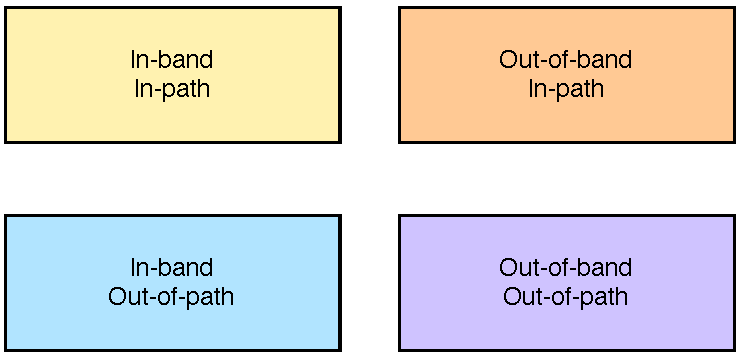
\includegraphics[width=0.9\columnwidth]{chap2-fw-outline}
\caption{Classification of Congestion cues~\cite{Singh:PhDFw}}
\label{fig:4:fw}
\end{figure}

A congestion control algorithm needs to pick one or more measurement points,
picking multiple adds to the feedback overhead and then choose a method to
signal it to the sending endpoint. It can choose to report it in-band by
encapsulating the cues either by piggybacking them on endpoint's own media
packets as RTP header extensions (this adds to the header overhead of a media
packet) or as RTCP extension blocks (see section~\ref{fw.freq} for details on
feedback frequency). Or the congestion control algorithm can choose to signal
the cues out-of-band, i.e., re-use the signaling path (e.g., SIP, XMPP) or
setup an alternate signaling path (e.g., HTTP or websockets). Following are
the examples for each category in the classification:

\textbf{\texttt{a) In-path, In-band}}: TFRC using information in RTCP RR, TFRC
using additional loss reported by ECN markings, Temporary Maximum Media Stream
Bit Rate Request (TMMBR), Receiver Estimated Max Bitrate (REMB).

\textbf{\texttt{b) In-path, Out-of-band}}: RTSP implements a SPEED parameter
to vary the transmission rate, announcing bandwidth in the SDP.

\textbf{\texttt{c) Out-of-path, In-band}}: Multipath RTP (congestion on one
path causes a change in the fractional distribution of traffic on each path.)

\textbf{\texttt{d) Out-of-path, Out-of-band}}: bandwidth/congestion
notifications from congestion maps, bandwidth lookup service, superpeers and
overlays.

% monitoring: long-term, short-term

% Additionally if the cue reliably
% describes the onset of congestion (\emph{knee}) or the collapse
% (\emph{cliff}).

% \begin{figure}[!h]
% 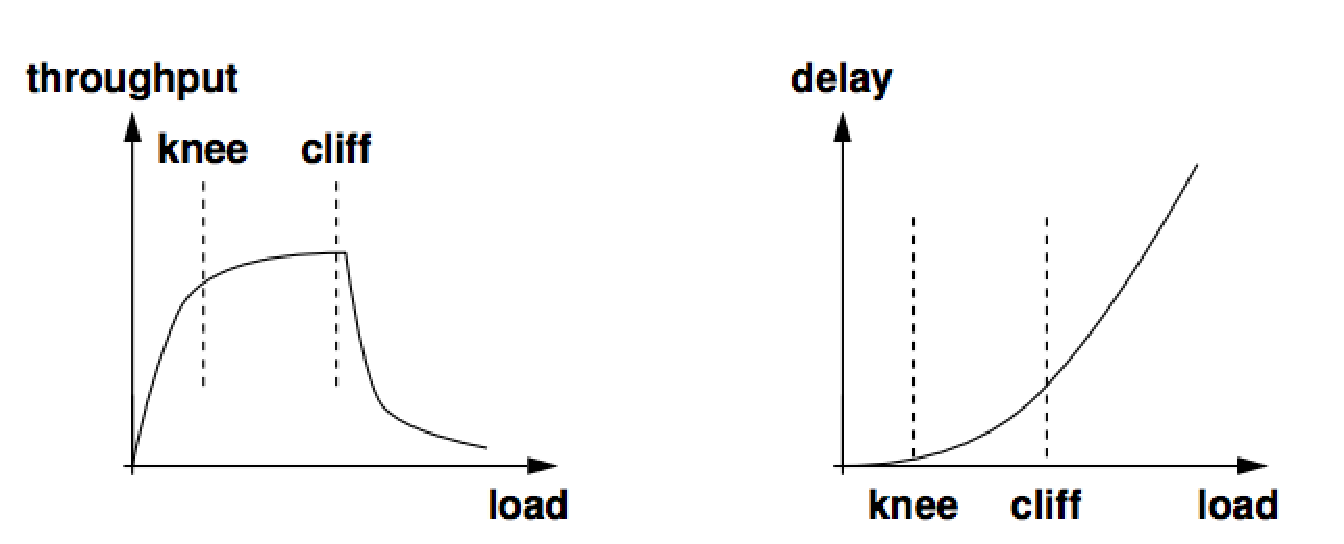
\includegraphics[width=\columnwidth]{chap4-knee-cliff}
% \caption{Shows the variation throughput and delay with increasing network load}
% \label{fig:4:knee}
% \end{figure}

\section{Congestion Control Evaluation}
\label{fw.cc.eval}

We need to define a set of requirements in order to design a congestion
control algorithm for multimedia. As a second step these requirements are used
as a checklist to evaluate the suitability of the proposed algorithms. Real-
time interactive communication differs greatly from \emph{elastic} traffic
because the sender generates media packets in real-time and expects it to be
delivered in 100s of milliseconds and the receiver consumes the media packets
almost immediately, hence late arriving packets are useless. Additionally,
real-time communication systems are able to tolerate some amount of packet
loss and adapt the media rate over a fairly large range.
\cite{draft.rmcat.req} lists a set of requirements for RTP-based interactive
multimedia sessions, these requirements form the basis of the guidelines
described in~\cite{draft.rmcat.evaluate}.  We define a catelogue of
\emph{traffic flows} traversing through a \emph{network topology} with varying
\emph{link characteristics} and diverse \emph{queuing} strategies. By picking
one feature from each category in the category, we construct scenarios to
evaluate the performance of the congestion control. The evaluation scenarios
are built using the following components: network topology, link and router
characteristics.

\subsection{Network flows}

\begin{enumerate}

\item \textbf{\texttt{Single media flow on an end-to-end path}}: this scenario
describes the best case, wherein the network puts each flow identified by its
5-tuple (protocol, source and destination IP address, source and destination
port numbers) on its own queue, thereby the flow using the proposed congestion
control algorithm does not encounter any cross-traffic.

\item \textbf{\texttt{Single media flow competing with the similar flows}}: in
this scenario, the flow using the proposed congestion control algorithm
competes with flows using the same congestion control algorithm (i.e., all
flows are interactive multimedia).


\item \textbf{\texttt{Single media flow competing with TCP}}: in this
scenario, the flow using the proposed congestion control algorithm competes
with TCP flows. These maybe \emph{short} TCP flows depicting common web-%
traffic patterns or \emph{long} TCP flows depicting bulk transfers (e.g.,
large file downloads).

\end{enumerate}

% In Section~\ref{rg.title}, we describe the network traffic scenarios to
% evaluate the proposed congestion control algorithms, namely, when the flows
% are a) alone, b) competing with self-similar flows, and c) competing with TCP
% flows (short-, long-lived) on a bottleneck link.

\subsection{Network topology}

\subsection{Link characteristics}

\subsection{Router characteristics}


% Flow scenarios
% Link properties
% Router properties